% Sample file for AES paper
\documentclass[fleqn]{jaes}

% Metadata Information
\jyear{2021}
\jmonth{June}
%\jvol{69}
%\jnum{3}

\usepackage{amsmath}\setlength{\mathindent}{10pt}
\usepackage{bm}
\usepackage{hyperref}
\usepackage{draftwatermark}
\SetWatermarkText{DRAFT}
\SetWatermarkColor[gray]{0.9}
\SetWatermarkScale{1.4}

\begin{document}

% Page heads
\markboth{MEIK\"AL\"AINEN AND DOE}{JAES TEMPLATE}


% Title portion
\title{Journal of the Audio Engineering Society Template\thanks{To whom correspondence should be addressed, e-mail: vesa.valimaki@aes.org. Last updated: June 28, 2021}}

%Author Info.
\authorgroup{
\author{MATTI MEIK\"AL\"AINEN,\textsuperscript{1}}
\role{AES Member,}
AND \author{JANE DOE,\textsuperscript{2}}
\role{AES Fellow}
\email{(matti.meikalainen@xyz.edu)\quad\quad\quad\quad\quad\quad\quad\quad\quad\quad\quad (jane\_doe@company.com)}
\affil{\textsuperscript{1}Acoustic Research Laboratory, Department of Sound Processing, XYZ University, City, Country \\
\textsuperscript{2}Audio Technology Company, City, State, USA}
}

%Abstract
\abstract{%
An informative and self-contained abstract of 100 to 200 words must be provided. The abstract should mention the motivation, problem statement, approach, results, and implications of the work, usually with one or two sentences each. It is recommended that the abstract be written in a single paragraph without citing any references. The Journal of the Audio Engineering Society is a modern scientific journal supporting online publishing with colors and a graphical abstract. It is a hybrid journal publishing both Open Access and traditional papers, the latter being only available for subscribers, such as AES members. If a paper published in the Journal of the Audio Engineering Society has been made Open Access, it will have the OA logo next to it and will be freely downloadable from the AES E-Library by anyone, even if they are not an AES member or E-Library subscriber. This example abstract contains 149 words.}
\maketitle
%Head 1
\section{INTRODUCTION}
The Journal of the Audio Engineering Society (JAES) seeks original unpublihed research papers and engineering reports of archive quality on subjects related to the audio domain. All submissions will go through a peer review process to check their suitability for JAES. Manuscripts should describe original work unpublished elsewhere and not being considered for publication elsewhere. The different types of possible submission are:
\begin{itemize}
    \item Research Paper
    \item Engineering Report
    \item Review Paper
    \item Communication
    \item Letter to the Editor
\end{itemize}
\noindent Full details of these submission types are given on the AES Journal Manuscript Types page: \url{https://www.aes.org/journal/authors/manuscript\_types/}. All articles accepted for publication will be subject to page fee charges, when the final length exceeds 10 pages. Please always refer to the web page Author Guidelines to be sure that you follow the newest rules: \url{https://www.aes.org/journal/authors/guidelines/}.

Authors should submit a manuscript for review to the online submission and peer-review system: \url{https://www.aes.org/journal/submit/}. Manuscripts are reviewed anonymously by members of the review board. After the reviewers’ analysis and recommendation to the editors, the author is advised of either acceptance or rejection. On the basis of the reviewers’ comments, the editor may request that the author make certain revisions which will allow the paper to be accepted for publication.

A growing number of JAES papers is published as Open Access articles. They are freely available to read for all, and not only to AES Members. This is certain to attract more readers and citations for these articles. The authors of each paper can decide whether they want their work to be available like this. The AES policy on Open Access is explained in detail on the Open Access web pages: \url{https://www.aes.org/openaccess/}.

The final paragraph of the Introduction should briefly summary the contents of the rest of the paper. Sec.~1 describes how the paper may be organized and how equations, figures, tables, and a graphical abstract are formatted. The reference format is described in Sec.~2. Sec.~3 gives instructions about author photographs and biographies. Sec.~4 lists the basic requirements for JAES papers, and Sec.~5 concludes. 

\section{ORGANIZATION}

Technical articles published in JAES should be informative and well organized. They should cite original work or review previous work, giving proper credit. Results of actual experiments or research should be included. The Journal cannot accept unsubstantiated or commercial statements. Authors should observe the general requirements for AES Publications, as agreed by the Publications Policy Committee, given in Sec.~4 of this template.

The paper title should be short, accurate, and exciting. It should give an idea of the type of work. For example, the title of a research paper should highlight the main application or advantage of the presented work. Similarly, a review article should have a broad and inclusive title. The paper title should include the essential keyword(s) to attract readers. The use of acronyms or uncommon words in the title is discouraged because they limit the number of potential readers. Words “new” and “novel” in the paper title are prohibited. Repeating a word in the title is not recommended.

The manuscript should develop the main point, beginning with a section entitled Introduction and ending with a Conclusion. Subheads are appropriate and should be inserted where necessary. Section division numbers should be of the form 0 (only for Introduction), 1, 1.1, 1.1.1, 2, 2.1, 2.1.1, etc. Paragraphs longer than 180 words and paragraphs containing a single sentence should be avoided.

Mathematical symbols, abbreviations, and acronyms, which may not be familiar to all readers must be spelled out or defined the first time they are cited in the text. Footnotes should be avoided, when possible, by making parenthetical remarks in the text.

Metric units according to the System of International Units (SI) should be used. For example, instead of 1 minute and 23 seconds, write 1 min and 23 s. Please use a space between the number and the unit, such as in 44.1\,kHz (not: 44.1kHz). Units are not generally italicized. When a number is used to count the number of cases, spell out numbers smaller than 10, for example “seven microphones” (not “7 microphones”) and “a five-point scale” (not “5-point”). 

\subsection{Equations}
This subsection shows how equations are inserted and formatted in a JAES article. A transfer function $A(z)$ can be written as
%Equation
\begin{equation}
A(z) = \frac{{a_1  + z^{ - 1} }}{{1 + a_1 z^{ - 1} }},
\label{eq:transfer_function}
\end{equation}

\noindent where $a_1$ and $a_2$ are variables, which should be italicized. They must be explained when they first appear. The equation should be part of the sentence in which it is inserted. Here is another equation, which ends a sentence: 

\begin{equation}
\phi (\omega ) =  - \omega  + 2 \arctan \left( {\frac{{a_1 \sin \omega }}{{1 + a_1 \cos \omega }}} \right).
\label{eq:phase_response}
\end{equation}
 
\noindent Function names, such as the trigonometric functions used in Eq.~\eqref{eq:phase_response} above, are not italicized. All equations should be numbered. This enables referring to them with their numbers, such as Eq.~\eqref{eq:transfer_function} and Eq.~\eqref{eq:phase_response} above. Bold characters for matrices can be written in the following way:
\begin{equation}
\mathbf{U}\mathbf{U}^\mathrm{H} = \mathbf{U}\mathbf{U}^\mathrm{H} = \mathbf{I}.
\end{equation}

\subsection{Figures}

 For the initial submission, illustrations should be incorporated in the same PDF as the manuscript, along with their captions, at a sufficiently high resolution for review purposes. It is recommended to produce all figures as EPS files or to covert them to EPS from other formats. LaTeX does not accept TIFF files. 
 
 Illustrations must have informative captions and must be referred to in the text, such as Fig.~\ref{fig:example_figure}. Figures presenting data must have a label on both the horizontal and the vertical axis, and the numerical scales and units must be indicated. A wide figure may expand over the two columns. Fig.~\ref{wide_figure} shows an example.

%Figure
\begin{figure}[t]
\centering
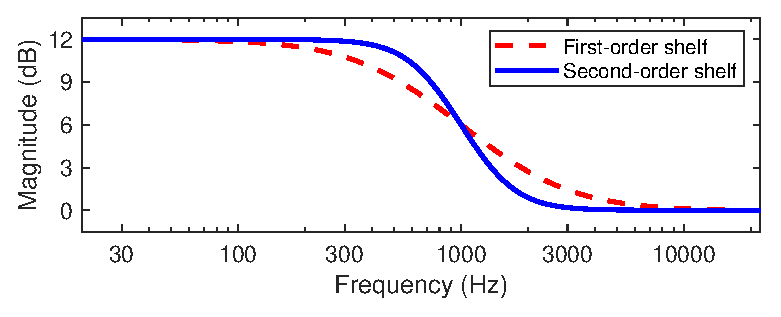
\includegraphics[width=82mm]{fig1_example.eps}
\caption{Figures using color must be understandable also in grayscale printing. It helps if both the line color and the line type are different for each curve.}
\label{fig:example_figure}
\end{figure}

For the final submission photographic and bitmapped images should be submitted as separate JPEG files with a resolution of at least 300 dpi. Line drawings can be submitted in EPS files. The figure number should be clearly indicated in the file name. The size of illustrations when printed in the Journal is usually 82 mm (3.25 inches) wide, although 170 mm (6.75 inches) wide can be used if required. 

Text labels on illustrations must be large enough so that the smallest letters are at least 1.5 mm (1/16 inch) high when the image is reduced to one of the above widths. If possible, text labels on all original illustrations should be scaled so that they will be the same size when reduced for reproduction in the Journal. Figure captions should either be inserted on a separate page of the main manuscript, following the references, or uploaded as a separate file. Captions should be concise.

Figures may publish online in full color; however, they will be converted to grayscale for print. Please review the figures and associated captions and legends/keys to ensure that figures will be understandable after being converted to black and white. For a fee, authors can choose to include color graphics files also in the printed version of the Journal.

\begin{figure*}
\centering
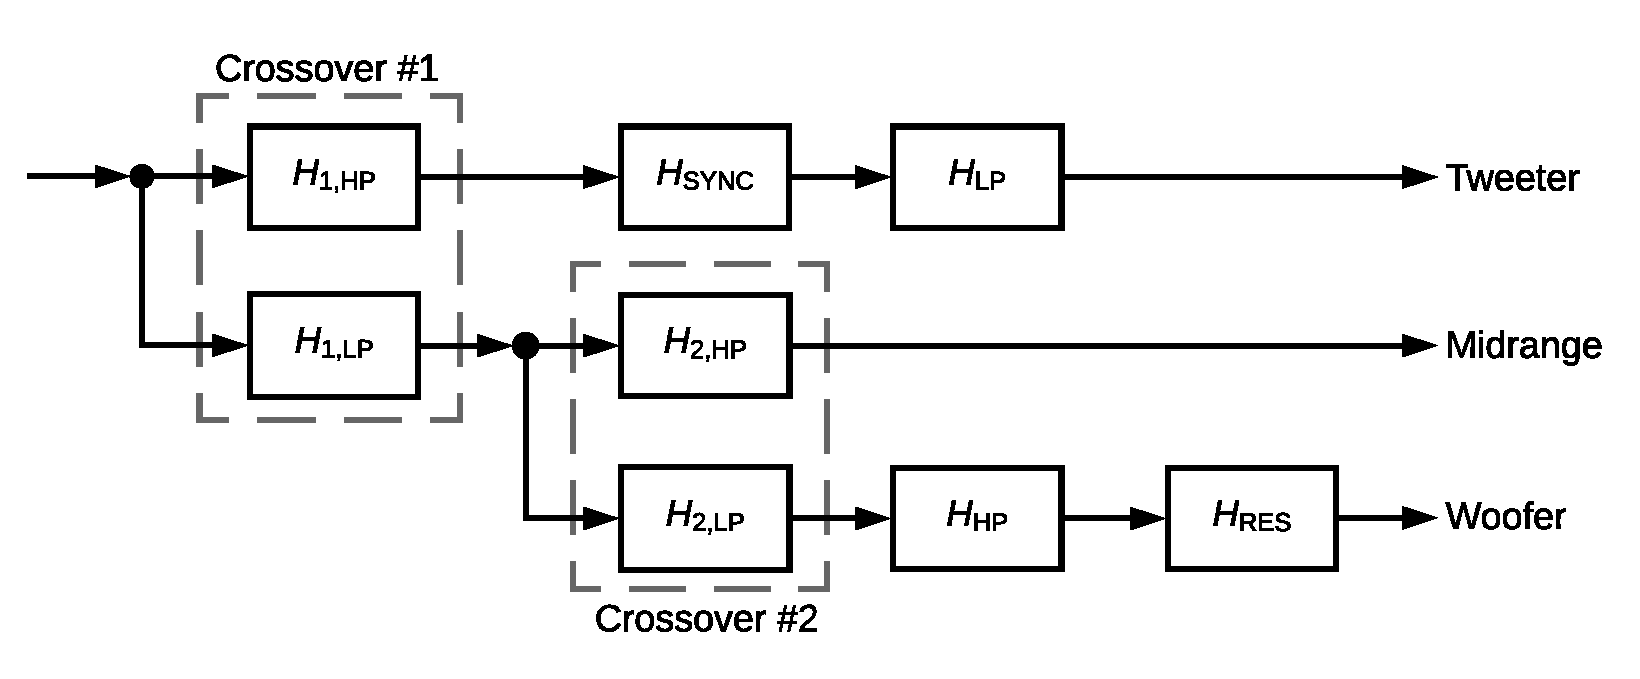
\includegraphics[trim=0cm 0.5cm 0cm 0.5cm, width=0.66\textwidth]{fig2_example.eps}
\caption{Example of a wide figure extending over the two columns.}
\label{wide_figure}
\end{figure*}

\subsection{Tables}

JAES articles often include tables, such as Table \ref{table:an_example_table}. They must be referred to and explained in text. 

%Table
\begin{table}[t]
\tabcolsep8.1pt
\caption{Tables should have a brief caption. Highlighting the best result(s) is helpful to readers.}
\label{table:an_example_table}
\\
 2 & Classical & FB   & 33\%\\
 3 & Jazz      & FF   & 76\%\\
 4 & Arabian   & FF   & 41\%\\
 5 & GNE       & H220 & 45\%\\
 6 & GNE       & H45  & 93\%\\
 7 & MNK       & G416 & 74\%\\
 8 & MNK       & D413 & 72\%\\
 9 & MNK       & R420 & \textbf{94\%}\\
10 & MNK       & N516 & 91\%\\\botrule
\end{tabular}}
\begin{tabnote}
Note. This table contains several acronyms which should be defined in the paper, when they are first used (but not in the abstract).
\end{tabnote}
\end{table}

\subsection{Graphical Abstract}
Authors of a paper accepted for publication in JAES are strongly encouraged to prepare a graphical abstract (GA) of the work performed. A GA is an image that summarises the work in an eye-catching way, ideally summarising the ideas of the paper. It appears alongside the text abstract in the online Journal and AES E-Library. The GA may be a figure from the article or preferably one specially prepared for the purpose\footnote{An example GA is available at: \url{https://www.aes.org/assets/base/img/content/journal/authors/guidelines/GraphicalAbstractExample4.png}}. A useful guide to preparing a GA can be found at \url{www.annaclemens.com/blog/make-graphical-abstract-paper}. 

Any text in the image should be clear and readable, in a sans serif font such as Helvetica or Arial. No caption or additional descriptive text is expected. The image file for the GA needs to be a PNG (Portable Network Graphics) file and should be uploaded with the final version of your manuscript. It should be in portrait format, US Letter or A4 aspect ratio, with a minimum resolution of 600 pixels wide, and preferably in color.

\section{REFERENCE FORMAT AND DOIS}
References should be cited numerically in brackets in order of appearance in the text. References should be listed at the end of the text in order of appearance. In the reference list, please insert “and” between the last and second-to-last author name. Use a comma before “and”, if there are more than two authors in the list. In publication titles, the first letters of the first word and the main words are capitalized in the paper title, but not prepositions and articles (see examples below).

References to periodicals (journals) should include the authors’ names, title of article, periodical title abbreviation, volume, issue number (optional), page numbers or article ID, year and month of publication, and the Digital Object Identifier (DOI) link, if available. The following are examples of the expected format of journal paper references \cite{a_journal_paper, a_journal_paper_with_many_authors, a_journal_paper_with_article_ID}.

Authors are expected to include DOIs for those references that have them, in the final version of their manuscripts, before a paper will be accepted for publication. Ideally, DOIs should be included for references when a paper is first submitted to us. The Journal is registered with CrossRef for the issuing of DOIs, and it is a condition of membership that we provide outbound linking of references in our papers. This enables readers to find the papers to which your references refer easily. We will also issue and register a DOI for your paper when it is published. Authors can look up individual DOIs using the free service provided by CrossRef here: \url{http://www.crossref.org/guestquery/} or for multiple references in a list using the text query interface at \url{http://www.crossref.org/SimpleTextQuery/} (you will have to validate your email address by setting up a free account).

Book references should contain the names of the authors, title of book, edition (if other than first), name and location of publisher, publication year, and page numbers \cite{a_book_ref, a_book_ref_2nd_edition}. A reference to a chapter published in an edited book should have the authors, the chapter name, the editors, the book title, the book series name, page numbers, the name and location of the publisher, publication year, and the edition number \cite{a_book_chapter}. 

For conference papers published in Proceedings, please include “in \emph{Proceedings of the}” in front of the conference name and spell out the full conference name. The conference acronym may optionally be shown in parentheses. The page numbers (if available), conference address (city, county/state), and year and month of publishing should also be shown, like in this example \cite{a_conference_paper}. The year of the conference is deleted from the conference name, if it is the same as the year of publishing. For this reason, this reference mentions the acronym “DAFx”, not “DAFx-17” \cite{a_conference_paper}. 

A slightly different format is used for AES convention papers and for abstract only presentations. After the paper title, insert “presented at the” before the number of the convention. The convention paper number can optionally be included, as in this example \cite{AES_convention_paper}. References to AES convention papers should be replaced with Journal publication citations if appropriately related Journal papers have been published.

For a thesis reference, please include the author name, thesis title, type of thesis (Ph.D. thesis or M.Sc. thesis), the name and address (city, country/state) of the university, year and, optionally, the month of publication. For example, this is a complete reference to a doctoral thesis \cite{a_PhD_thesis} and this a reference to a Master's thesis \cite{an_MSc_thesis}. 

References to a patent should include the inventors’ names, patent title, specification of the patent (e.g. US or European patent) together with the patent number, and year and month of publication. The following is an example of the expected format of a patent reference in JAES \cite{a_patent}. 

A web page reference should include the author, such as a company, the title of the web page, the web address (URL), and the date accessed. This is an example of a correctly referenced web site in JAES \cite{a_web_page}. More examples of our current reference style may be viewed in recent issues of JAES.

\section{AUTHOR PHOTOGRAPHS AND BIOGRAPHIES}
Author photographs and biographies are required for each author for all research papers, engineering reports, and review papers. Each photograph should be a professional photo of the author’s face and the image must be able to be supplied as a separate, high-resolution graphic (TIFF, EPS, or JPEG files with a resolution of at least 300 dpi). 

Author biographies should highlight each author’s education, places of employment, research visits, key research areas, professional memberships, and awards in 150 words or less. This section should appear after the references at the end of the manuscript file. Examples are given at the end of this template.


\section{GENERAL REQUIREMENTS}
All material published by the AES, regardless of the type, shall conform to the following requirements unless specifically exempted by Publications Policy or by the Editor.

\begin{itemize}
    \item Style: The technical content should be accurate; the writing should use good grammar and be easy to understand by those versed in the art. Abbreviations, units, and definitions of quantities should conform to the AES editorial style.
    
    \item Good Taste: Good taste is a necessity. No derogatory mention of other engineering work, engineers, or organizations shall be made. (Constructive technical criticism, which makes a suggestion(s) for improvement(s) that would remove the objection, is not derogatory if the technical basis is well developed and accurate.) The Editorial Office should ask reviewers to judge carefully the substance of such criticism. Specifically, the initiation of controversy should be minimized by a careful checking of the critical judgments. Controversy for its own sake should be discouraged.
    
    \item Commercialism: A manuscript which is based on a commercial product should be reviewed extremely carefully to determine the real scientific content. If a manuscript has no other merit than as a description of the product, it is not acceptable. This requirement is especially important in articles that provide technical results without an adequate description of a device’s operation.
    
    \item Original unpublished work: Manuscripts should describe original work unpublished elsewhere and not being considered for publication elsewhere. The Editor may also reject manuscripts that are original, but too similar to other published work. Publications of AES meetings, or of other meetings at the discretion of the Editor, may be further reviewed and republished in JAES, but only after they been revised and extended.
    
    \item Trademarks: Trademarks are generally inappropriate because they serve a commercial purpose, not an engineering purpose. a) Trademark symbols are not permitted. b) Trademark names in titles and abstracts should be replaced by generic descriptions where possible. If trademarked names are retained in titles and abstracts, they will not be acknowledged as such. c) The first time a trademarked name appears in the body text, it may be footnoted. The footnote will state that it is registered and the name of the owner.
\end{itemize}

\section{CONCLUSION}
The manuscript submitted to JAES should end with a section entitled Conclusion. The Conclusion should briefly review the main points of the paper. However, do not replicate the abstract. All results mentioned in the Conclusion must be deducted from the other parts of the paper. Do not introduce new results in the Conclusion. This section may also speculate on applications and extensions of the results (future work). Many readers browsing technical papers only read the abstract and the Conclusion.

\section{ACKNOWLEDGMENT}
This  work  has  been  funded  in  part  by  the  Academy of   Finland   (project no.~654321). This template version was edited by Kurt James Werner and Vesa V\"alim\"aki. 

% - If you are using bibTex for references, you need these lines: 
%\bibliography{jaes.bib}
%\bibliographystyle{jaes.bst}

% NOTE:
% - in case you are not using bibTex you have to manually edit the bibliograpy as below.
%%%%%%%%%%%%%%%%%%%%%%%%%%%%%%%%%%
\begin{thebibliography}{99}

\newcommand{\enquote}[1]{``#1''}
\providecommand{\url}[1]{\texttt{#1}}
\providecommand{\urlprefix}{URL }
\expandafter\ifx\csname urlstyle\endcsname\relax
  \providecommand{\doi}[1]{[Online]. Available: %\discretionary{}{}{}#1}\else
  \providecommand{\doi}{doi:\discretionary{}{}{}\begingroup
  \urlstyle{rm}\Url}\fi

\bibitem{a_journal_paper}
Y.~Li, J.~Cai, Q.~Dong, L.~Wu, and Q.~Chen, \enquote{Psychophysiological Responses of Young People to Soundscapes in Actual Rural and City Environments,} \emph{J. Audio Eng. Soc.}, vol. 68, no. 11, pp. 910–925 (2020 Dec.), https://doi.org/10.17743/jaes.2020.0060.

\bibitem{a_journal_paper_with_many_authors}
T.~Fujioka, C.~Freigang, K.~Honjo, J.~J.~Chen, J.~L.~Chen, S.~E.~Black, \emph{et al.}, \enquote{Central Auditory Processing in Adults with Chronic Stroke Without Hearing Loss: A Magnetoencephalography Study,} \emph{Clin. Neurophysiol.}, vol. 131, no. 5, pp. 1102–1118 (2020 May), https://doi.org/10.1016/j.clinph.2020.01.014.

\bibitem{a_journal_paper_with_article_ID}
S.~Ntalampiras, I.~Potamitis, and~N.   Fakotakis, \enquote{Exploiting Temporal Feature Integration for Generalized Sound Recognition,} \emph{EURASIP J. Adv. Signal Process.},  vol. 2009, no. 1, paper 807162  (2009 Dec.), https://doi.org/10.1155/2009/807162.

\bibitem{a_book_ref}
V.~Pulkki and  M.~Karjalainen, \emph{Communication Acoustics: An Introduction to Speech, Audio and Psychoacoustics} (Wiley, Chichester, UK, 2015).

\bibitem{a_book_ref_2nd_edition}
D.~Oram, \emph{An Individual Note of Music, Sound and Electronics}, 2nd ed. (Anomie Academic, Swindon, UK, 2016).

\bibitem{a_book_chapter}
V.~V\"alim\"aki,  S.~Bilbao,  J.~O.~Smith,  J.~S.~Abel, J.~Pakarinen, and D.~Berners, \enquote{Virtual Analog Effects,} in U. Z\"olzer (Ed.), \emph{DAFX---Digital Audio Effects},  pp. 473--522 (John Wiley \& Sons, Chichester, UK, 2011), 2nd ed.

\bibitem{a_conference_paper}
S.~J.~Schlecht and E.~A.~Habets, \enquote{Accurate Reverberation Time Control in Feedback Delay Networks,} in \emph{Proceedings of the International Conference on Digital Audio Effects (DAFx)}, pp. 337--344 (Edinburgh, UK) (2017 Sep.).

\bibitem{AES_convention_paper}
M.~Gospodarek, A.~Genovese, D.~Dembeck, C.~Brenner,  A.~Roginska, and K.~Perlin, \enquote{Sound  Design  and Reproduction Techniques for Co-Located Narrative  VR Experiences,} presented  at  the \emph{147th Convention of the Audio Engineering Society} (2019 Oct.), paper 10287.

\bibitem{a_PhD_thesis} 
P.~D.~L.~G.~Pestana, \emph{Automatic Mixing Systems Using Adaptive Digital Audio Effects}, Ph.D. thesis, Universidade Cat\'olica Portuguesa, Porto, Portugal (2013 Feb.).

\bibitem{an_MSc_thesis}
J.~Holm, \emph{Applying the Finite Element Method for Modelling Loudspeaker Waveguide Directivity},  Master’s thesis, Aalto University, Espoo, Finland (2010 May).

\bibitem{a_patent}
P.~G.~Craven and  M.~A.~Gerzon, \enquote{Coincident  Microphone Simulation Covering Three Dimensional Space and Yielding Various Directional Outputs,}  US Patent 4,042,779 (1977 Aug.).

\bibitem{a_web_page}
Audio Engineering Society, \enquote{Journal Author Guidelines,} https://www.aes.org/journal/authors/guidelines/ (accessed Mar. 9, 2021).

\end{thebibliography}
%%%%%%%%%%%%%%%%%%%%%%%%%%%%%%%%%%

\break

%Appendix
\appendix

\section*{APPENDIX}
One or more Appendices can appear after the references. An Appendix can present for example a mathematical derivation, pseudo-code, or other additional data, which is unsuitable to show in the body of the article.

%Biography
 \biography{Matti Meik\"al\"ainen}{headshot1.jpg}{Matti Meik\"al\"ainen is Professor of audio technology at XYZ University, Espoo, Finland. He received his M.Sc. and Ph.D.~degrees from Helsinki University of Technology in 1992 and in 1995, respectively. In 1996, he was a postdoctoral research fellow at the University of Westminster, London, UK. In 2001--2002, he was Professor of signal processing at the Pori School of Technology and Economics, Tampere University of Technology, Pori, Finland. In 2008--2009, he was a visiting scholar at the Center for Computer Research in Music and Acoustics (CCRMA), Stanford University, Stanford, CA. His research interests include musical signal processing, digital filter design, and acoustics of musical instruments. Prof. Meik\"al\"ainen is a senior member of the IEEE and is a member of the Acoustical Society of Finland. He was the Chair of the 11th International Conference on Digital Audio Effects (DAFx), which was held in Espoo, Finland, in 2008.}
 
 \biography{Jane Doe}{headshot2.jpg}{Jane Doe is a Consulting Professor at the Center for Computer Research in Music and Acoustics (CCRMA) in the Music Department at Stanford University where her research interests include audio and music applications of signal and array processing, parameter estimation, and acoustics. She holds Ph.D.~and M.S.~degrees from Stanford University, and an S.B.~from MIT, all in electrical engineering. Dr.~Doe was a researcher at NASA/Ames Research Center, exploring topics in room acoustics and spatial hearing on a grant through the San Jose State University Foundation. She was also chief scientist of Crystal River Engineering, Inc., where she developed their positional audio technology, and a lecturer in the Department of Electrical Engineering at Yale University. Dr.~Doe is a Fellow of the Audio Engineering Society.}
\end{document}
